%! TEX root = part8.tex
% the main TeX file which is intended to compile, :VimtexReload after adjustment
% :h vimtex-tex-root
\documentclass[../gbr_teknik.tex]{subfiles}
% \includeonlyframes{current}
% \setbeameroption{hide notes} % Only slides
% \setbeameroption{show only notes} % Only notes
\setbeameroption{show notes on second screen=right} % Both

\begin{document}

\section{Gambar Mur Baut}
\label{sec:gambar_mur_baut}

\begin{frame}[mytitle=center,c,mybg=bglight3,light]
	\frametitle{Tugas Kelas}
	\rtxt{digiPH_red}{digiPH_white}{Buatlah gambar \huge pandangan depan, atas dan samping kanan benda ``Mur-Baut" \normalsize di bawah ini pada kertas A4.}
	% Pada gambar cantumkan tanda pengerjaan dan toleransinya.
	\limg{tugas_mur}
\end{frame}

\begin{frame}[mytitle=standard,t,mycolor=digiPH_white,light]\frametitle{Tujuan}
	Setelah mempelajari bahan dalam bab ini, seharusnya Anda dapat:
	\begin{itemize}
		\item Menjelaskan perbedaan gambar ulir luar (baut) dan ulir dalam (mur).
		\item Menggambar ulir luar dan ulir dalam.
		\item Menghitung dimensi mur-baut.
		\item Mendesain gambar mur-baut.
	\end{itemize}\end{frame}

\begin{frame}[mytitle=standard,c,mybg=bglight2,light]\frametitle{Ulir Luar dan Ulir Dalam}
	\ltxt{digiPH_gray}{digiPH_darkblue}{Dalam gambar teknik mesin hampir setiap saat selalu ada gambar ulir. Untuk itu juru gambar dan teknisi di industri harus memiliki pengetahuan tentang tipe, penggunaan ulir, serta metode penggambarannya.}

	\rtxt{digiPH_gray}{digiPH_darkblue}{\begin{itemize}
			\item Ulir luar: diameter luar garis tebal, diameter dalam garis tipis
			\item Ulir dalam: diameter luar garis tipis, diameter dalam garis tebal
			\item Pandangan depan:
			      \begin{itemize}
				      \item Ulir luar: 3/4 lingkaran diameter dalam
				      \item Ulir dalam: 3/4 lingkaran diameter luar
			      \end{itemize}
		\end{itemize}}
\end{frame}


\begin{frame}[mytitle=standard,c,mycolor=digiPH_white,light]
	\frametitle{Gambar Ulir}
	\begin{center}
		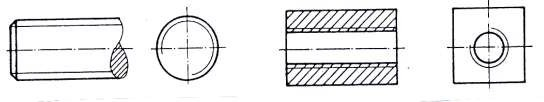
\includegraphics[width=.82\textwidth]{../figures/gbr_ulir.jpg}
	\end{center}\end{frame}

\begin{frame}[mytitle=standard,c,mybg=bglight2,light]
	\frametitle{Bentuk Ujung Baut}
	\begin{itemize}
		\item Ujung baut dapat digambar dalam dua bentuk:
		      \begin{itemize}
			      \item Lengkungan (radius = diameter luar baut)
			      \item Chamfer (sudut 45$^\circ$)
		      \end{itemize}
	\end{itemize}
\end{frame}

\begin{frame}[mytitle=standard,t,mybg=bglight2,light]
	\frametitle{Bentuk Ujung Baut}
	\begin{center}
		
\includegraphics[width=.72\textwidth]{ujung_baut}
	\end{center}\end{frame}

\begin{frame}[mytitle=standard,t,mycolor=digiPH_gray,light]\frametitle{Gambar Pasangan Mur-Baut}
	\ltxt{digiPH_gray}{digiPH_black}{\begin{itemize}
			\item Harus jelas agar mudah dibaca
			\item Umumnya cukup pandangan depan
			\item Bisa ditambah:
			      \begin{itemize}
				      \item Pandangan atas
				      \item Pandangan samping
			      \end{itemize}
			\item Bagian utama:
			      \begin{itemize}
				      \item Baut
				      \item Kepala baut
				      \item Mur
			      \end{itemize}
			\item Bentuk kepala: segi empat / segi enam
		\end{itemize}}

	\rimg{gbr_baut}
\end{frame}

%====================================================

\section{Gambar Roda Gigi}
\label{sec:Gambar Roda Gigi}

\begin{frame}[mytitle=standard,t,mycolor=digiPH_purple,dark]\frametitle{Tujuan}
	Setelah mempelajari bahan dalam bab ini, seharusnya Anda dapat:
	\begin{itemize}
		\item Menunjukkan cara menggambar roda gigi
		\item Mengidentifikasi macam-macam roda gigi
		\item Membaca dan menggambar roda gigi
	\end{itemize}\end{frame}

\begin{frame}[mytitle=standard,t,mybg=bglight2,light]
	\frametitle{Cara Menggambar Roda Gigi}
	\ltxt{digiPH_ocean}{digiPH_white}{Roda gigi adalah elemen mesin untuk meneruskan gerak dan daya.

		\begin{itemize}
			\item Dapat mempercepat atau memperlambat putaran
			\item Digambar secara sederhana sebagai roda pejal
		\end{itemize}}

	\rtxt{digiPH_ocean}{digiPH_white}{\begin{itemize}
			\item Lingkaran kepala: garis tebal
			\item Lingkaran jarak: garis sumbu tipis
			\item Lingkaran kaki: garis tipis (opsional)
			\item Gigi miring: ditunjukkan garis tipis arah gigi
		\end{itemize}}
\end{frame}

\begin{frame}[mytitle=center,c,mycolor=digiPH_white,light]
	\begin{center}
		
\includegraphics[width=.82\textwidth]{gbr_roda_gigi}
	\end{center}
\end{frame}

\begin{frame}[mytitle=center,t,mybg=bglight3,light]
	\frametitle{Macam Pasangan Roda Gigi}
	\txt{digiPH_red}{digiPH_white}{\begin{itemize}
			\item Roda gigi lurus
			\item Roda gigi cacing
			\item Roda gigi kerucut
			\item Roda gigi batang (rack)
			\item Roda gigi dalam
		\end{itemize}}
\end{frame}

\begin{frame}[mytitle=standard,t,mycolor=digiPH_uniblue,light]
	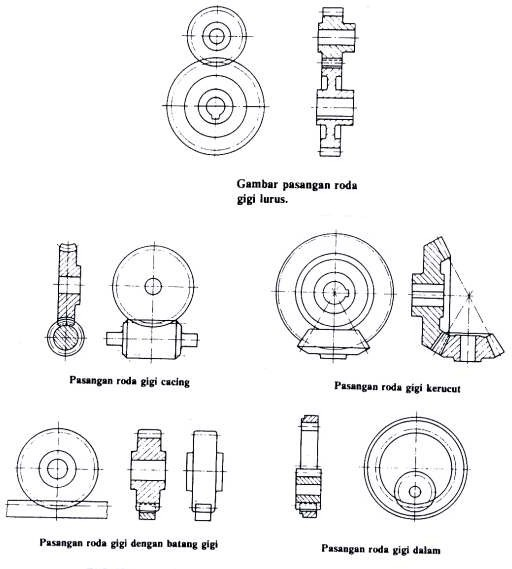
\includegraphics[height=.85\textheight]{../figures/macam_roda_gigi}
\end{frame}

\end{document}
